\chapter{Methodology}
\label{Methodology}

% mention ethics approval

All programming for this dissertation was written in Python \cite{python} and the source code is accessible on \href{https://github.com/zakdux/counter-strike}{GitHub}.

\section{Data Collection}

\href{https://www.hltv.org/}{HLTV} is a household name in the Counter-Strike scene. Since its inception in 2002, it has evolved from a repository of CS 1.6 match recordings to a hub for all things Counter-Strike: fixtures, news articles, player interviews, and much more complement an enormous public database of match statistics. 

Every professional and most semi-pro teams are tracked on HLTV; an extensive array of statistics for every match played at every tournament is reported. Furthermore, game play recordings, known as demo files, are hosted for the majority of high-level matches. These demo files can be downloaded and replayed to recreate each second of a given match.

\href{https://liquipedia.net/counterstrike/}{Liquipedia} is a viable alternative to HLTV; it is a collaborative online encyclopedia (a wiki) with records dating back to the very first CS tournament. Ultimately, HLTV was selected for its easy-to-navigate interface and increased depth of statistical data. Unlike Liquipedia, however, HLTV does not provide an API for retrieving the match data at scale. Thus a web-scraping solution is required. A web-scraper is a program which can automatically request, download, and parse information from web pages.

\subsection{Requirements}

The development requirements for data collection were therefore to:

\begin{enumerate}
\item{Design a database to store desired match, map, and player data}
\item{Automatically download relevant match pages from HLTV}
\item{Parse information from the pages and store it in a database}
\item{Synchronize the database with the latest HLTV data}
\end{enumerate}

The following Python packages were identified as suitable for meeting these requirements:
\begin{itemize}
\item{\textbf{SQLAlchemy}, for object-relational mapping to a \textbf{SQLite} database}
\item{\textbf{ZenRows}, for efficiently downloading pages from HLTV}
\item{\textbf{BeautifulSoup}, for reading and extracting data from downloaded pages}
\end{itemize} 


\subsection{Database design}

%The database should be designed to comprehensively store historic match information. This means that it can include details about each match, which maps were played, which players played on each team, and how well they performed. The table schemas were designed by observing which information on the HLTV pages are relevant.

\subsubsection{Matches}

Every professional game of Counter-Strike is represented on HLTV by means of a \textbf{match} page. These list a wealth of information, such as the teams playing, the maps played, and the map veto sequence. There are also links to watch recordings of the match or download the demo file. An example of a match page is shown in Figure \ref{fig:match_cropped}. The schema shown in Table \ref{tab:match} was determined after considering which data on the match page is relevant to the project.

\begin{figure}[h]
	\centering
	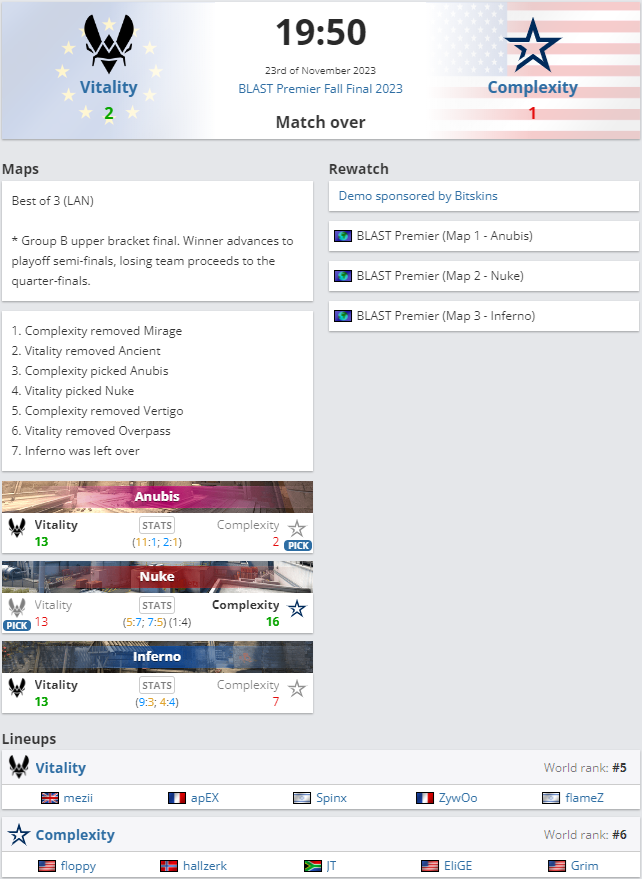
\includegraphics[width=0.9\textwidth]{Figures/hltv/match-cropped-3.png}
	\caption{An HLTV \href{https://www.hltv.org/matches/2368036/vitality-vs-complexity-blast-premier-fall-final-2023}{match page} for Vitality versus Complexity (cropped)}
	\label{fig:match_cropped}
\end{figure}

\begin{table}[h!]
	\centering
	\caption{Simplified schema for the \texttt{match} table}
	\renewcommand{\arraystretch}{1.2} % Adjust vertical spacing
	\begin{tabular}{|>{\ttfamily}l|>{\ttfamily}c|l|}
		\hline
		\multicolumn{1}{|c|}{\textnormal{\textbf{Field}}} & \multicolumn{1}{c|}{\textnormal{\textbf{Type}}} & \multicolumn{1}{c|}{\textbf{Description}} \\
		\hline
		id & INTEGER & Match ID, the primary key\\
		\hline
		datetime & DATETIME & Date and time at start of match\\
		\hline
		team1\_id & INTEGER & Identifier for the first team \\
		\hline
		team2\_id & INTEGER & Identifier for the second team \\
		\hline
		team1\_score & INTEGER & Number of maps\footnotemark[1] won by first team \\
		\hline
		team2\_score & INTEGER & Number of maps\footnotemark[1] won by second team \\
		\hline
		event\_id & INTEGER & Identifier for the event\\
		\hline
		event & STRING & Name of the event\\
		\hline
		lan & BOOLEAN & Indicates if the match was played on a LAN or online\\
		\hline
		best\_of & INTEGER & The match format (1/3/5)\\
		\hline
		box\_str & STRING & Extra details reported on match page\\
		\hline
		veto & STRING & The order of the map veto process\\
		\hline
		cs2 & BOOLEAN & Indicates if match was played in CS2 or CS:GO \\
		\hline
	\end{tabular}
	\label{tab:match}
\end{table}

\newpage

The five players that make up each team are reported at the bottom of every match page in the 'Lineup' section. This information is useful to record as rosters change over time and players are sometimes substituted. It was thus decided to record the two line-ups for every match in a separate table. This schema is shown in Table \ref{tab:lineup}.

\begin{table}[h!]
	\centering
	\caption{Simplified schema for the \texttt{lineup} table}
	\renewcommand{\arraystretch}{1.2} % Adjust vertical spacing
	\begin{tabular}{|>{\ttfamily}l|>{\ttfamily}c|l|}
		\hline
		\multicolumn{1}{|c|}{\textnormal{\textbf{Field}}} & \multicolumn{1}{c|}{\textnormal{\textbf{Type}}} & \multicolumn{1}{c|}{\textbf{Description}} \\
		\hline
		id & INTEGER & Lineup ID, the primary key \\
		\hline
		team\_id & INTEGER & Identifier for the team \\
		\hline
		rank & INTEGER & HLTV team rank at that time \\
		\hline
		match\_id & INTEGER & Identifier for the associated match \\
		\hline
		player1\_id & INTEGER & Identifier for the first player \\
		\hline
		player2\_id & INTEGER & Identifier for the second player \\
		\hline
		player3\_id & INTEGER & Identifier for the third player \\
		\hline
		player4\_id & INTEGER & Identifier for the fourth player \\
		\hline
		player5\_id & INTEGER & Identifier for the fifth player \\
		\hline
	\end{tabular}
	\label{tab:lineup}
\end{table}

\footnotetext[1]{In a BO1, the score is the number of rounds won}
\clearpage

\subsubsection{Maps}

\label{maps}

Clicking on any of the individual map results listed on the match page will load the \textbf{map} page. These pages report more granular data for  each map that was played in the match. A BO3 match, for example, consists of either two or three maps, all of which will have their own map page with detailed statistics. An example of a map page is shown in Figure \ref{fig:map_cropped}, which was retrieved by clicking on the 'STATS' button on the corresponding tile on the match page. The schema shown in Table \ref{tab:map} was determined after considering which data on the match page is relevant to the project.

\begin{figure}[h!]
	\centering
	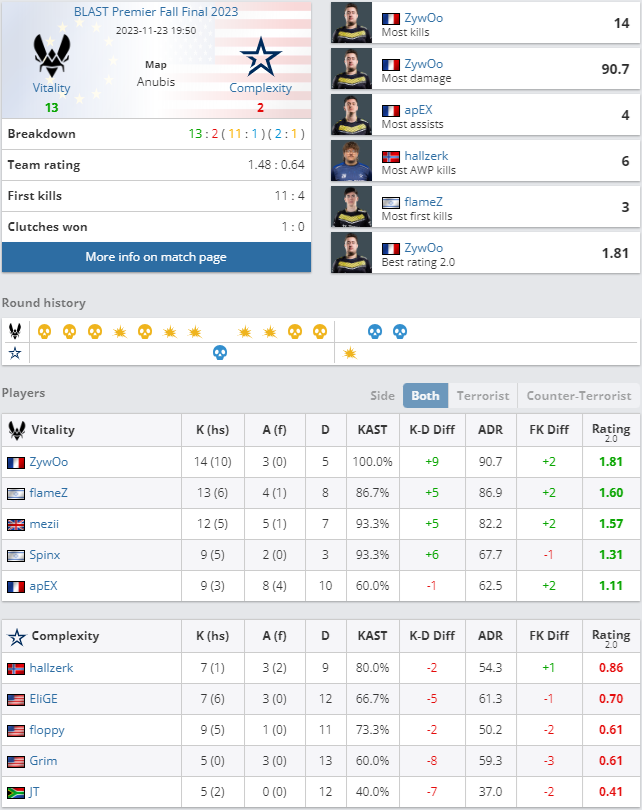
\includegraphics[width=0.9\textwidth]{Figures/hltv/map-cropped-2.png}
	\caption{A \href{https://www.hltv.org/stats/matches/mapstatsid/167162/complexity-vs-vitality}{map page} for the first map played, Anubis, in the match between Vitality and Complexity (cropped)}
	\label{fig:map_cropped}
\end{figure}

\clearpage

\begin{table}[h]
	\centering
	\caption{Simplified schema for the \texttt{map} table}
	\renewcommand{\arraystretch}{1.2} % Adjust vertical spacing
	\begin{tabular}{|>{\ttfamily}l|>{\ttfamily}c|l|}
		\hline
		\multicolumn{1}{|c|}{\textnormal{\textbf{Field}}} & \multicolumn{1}{c|}{\textnormal{\textbf{Type}}} & \multicolumn{1}{c|}{\textbf{Description}} \\
		\hline
		id & INTEGER & Map ID, the primary key \\
		\hline
		match\_id & INTEGER & Identifier for the match \\
		\hline
		t1\_id & INTEGER & Identifier for Team 1 \\
		\hline
		t2\_id & INTEGER & Identifier for Team 2 \\
		\hline
		map\_name & STRING & Name of the map \\
		\hline
		t1\_score & INTEGER & Rounds won by team 1\\
		\hline
		t2\_score & INTEGER & Rounds won by team 2\\
		\hline
		t1\_rating & FLOAT & Team 1 HLTV rating \\
		\hline
		t2\_rating & FLOAT & Team 2 HLTV rating \\
		\hline
		t1\_first\_kills & INTEGER & Team 1 first kills \\
		\hline
		t2\_first\_kills & INTEGER & Team 2 first kills \\
		\hline
		t1\_clutches & INTEGER & Team 1 clutches\footnotemark[2] \\
		\hline
		t2\_clutches & INTEGER & Team 2 clutches\footnotemark[2] \\
		\hline
		t1\_round\_history & STRING & Team 1 round outcomes \\
		\hline
		t2\_round\_history & STRING & Team 2 round outcomes \\
		\hline
	\end{tabular}
	\label{tab:map}
\end{table}


\footnotetext[2]{A clutch is when all of a player's teammates are eliminated and they still win the round}

Each player's \textbf{performance} on a given map is reported on the table on the map page. Their performance is measured by a number of statistics, such as their kill-death ratio (KDR), average damage per round (ADR), and flashbang assists. These are described in table \ref{tab:playerstats}.

\begin{table}[h!]
	\centering
	\caption{Simplified schema for the \texttt{playerstats} table}
	\renewcommand{\arraystretch}{1.2} % Adjust vertical spacing
	\begin{tabular}{|>{\ttfamily}l|>{\ttfamily}c|l|}
		\hline
		\multicolumn{1}{|c|}{\textnormal{\textbf{Field}}} & \multicolumn{1}{c|}{\textnormal{\textbf{Type}}} & \multicolumn{1}{c|}{\textbf{Description}} \\
		\hline
		player\_id & INTEGER & Player ID, part of the composite primary key \\
		\hline
		map\_id & INTEGER & Map ID, part of the composite primary key \\
		\hline
		kills & INTEGER & Number of kills by the player \\
		\hline
		hs & INTEGER & Number of headshot kills \\
		\hline
		assists & INTEGER & Number of assists by the player \\
		\hline
		flashes & INTEGER & Number of times a thrown flashbang led to a kill \\
		\hline
		deaths & INTEGER & Number of player deaths \\
		\hline
		kast & FLOAT & Kill/Assist/Survival/Traded (KAST) percentage \\
		\hline
		adr & FLOAT & Average damage per round in hit points \\
		\hline
		first\_kd & INTEGER & Number of times the player got the opening kill\\
		\hline
		rating & FLOAT & HLTV rating \\
		\hline
	\end{tabular}
	\label{tab:playerstats}
\end{table}

\newpage

\subsection{Downloading \& processing}

In order to populate the tables listed in the previous section, the web pages first needed to be downloaded and processed. By separating the scraping process into two discrete steps, downloading and processing, subsequent modifications could be made to the database and processing without the need to request any page data from HLTV a second time. 

The ZenRows package was used to great effect to download the data from HLTV. Many modern websites, including HLTV, make use of Cloudflare and other services to protect against cyberattacks and other malicious traffic. This results in inconsistent responses when issuing requests programmatically. By issuing the requests via the ZenRows API, the rate of successful responses was over 99\%. 

Due to the sheer magnitude of pages of data, concurrency was implemented to vastly improve the rate at which pages could be downloaded and processed. A function was written which initiates ten ZenRows API client instances, loops through the list of URLs, requests each one, and downloads the HTML data in each response. 

The next problem to solve was how to obtain the list of addresses for all the map- and match-pages.

\subsubsection{Finding the map links}

HLTV conveniently has a \href{https://www.hltv.org/stats/matches}{results page} that lists every single map in their database. An example of such a page is shown in Figure \ref{fig:map_urls}. The list can be filtered by event type (Majors, Big events, LAN, or online), date, ranking (where at least one of the teams playing must be ranked in the Top $x$ teams), and Map (Inferno, Mirage, etc.). By navigating through this list, all the desired links to the map pages could be retrieved. This page will henceforth be referred to as the \textit{map-link} page.

\begin{figure}[h]
	\centering
	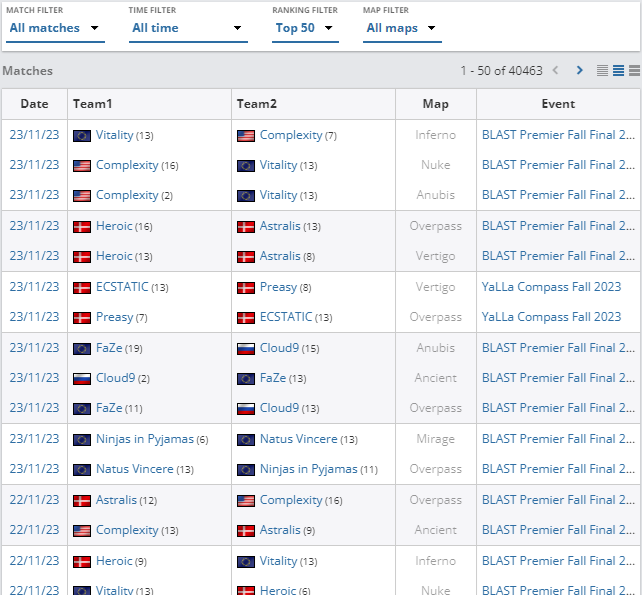
\includegraphics[width=0.9\textwidth]{Figures/hltv/map-urls-cropped-2.png}
	\caption{A map-link \href{https://www.hltv.org/stats/matches?startDate=all&rankingFilter=Top50}{page}, where each row is linked to a different map page}
	\label{fig:map_urls}
\end{figure}

Two noteworthy decisions were made here: to only record data from the last five years (from 2019 to the present), and to only consider matches where at least one of the teams was ranked in the Top 50 teams as reported by HLTV's weekly rankings. This was done to narrow the scope to relatively recent matches played by professional teams.

Each map-link page reports a maximum of 50 map records, which means that the scraper needs to be able to navigate through multiple pages, depending on the amount of rows, to retrieve all the URLs. This was done by downloading the first page, then processing it to find the pagination range. This range was then used to form the list of remaining pages to download.

Once all the map-link pages had been downloaded, the list of URLs to the map pages themselves needed to be extracted. Each file was sequentially processed to isolate the map ID and URL for each map played. Further details could be collected later when the map pages themselves were scraped. This information was stored in its own table, \texttt{map\_url}, along with two flags indicating if the respective map page had been downloaded and whether the map statistics had been processed and stored in the database.

\begin{table}[h]
	\centering
	\caption{Schema for the \texttt{map\_url} table}
	\renewcommand{\arraystretch}{1.2} % Adjust vertical spacing
	\begin{tabular}{|>{\ttfamily}l|>{\ttfamily}c|l|}
		\hline
		\multicolumn{1}{|c|}{\textnormal{\textbf{Field}}} & \multicolumn{1}{c|}{\textnormal{\textbf{Type}}} & \multicolumn{1}{c|}{\textbf{Description}} \\
		\hline
		id & INTEGER & Map ID, the primary key \\
		\hline
		url & STRING & The unique string in the map page URL \\
		\hline
		downloaded & BOOLEAN & Flag indicating if the page has been downloaded \\
		\hline
		processed & BOOLEAN & Flag indicating if the page has been processed \\
		\hline
	\end{tabular}
	\label{tab:map-link}
\end{table}


\newpage
\subsubsection{Downloading the maps and matches}
Once the list of map URLs was recorded, the individual map pages could be downloaded. An example of a map page is shown in Figure \ref{fig:map_cropped}. The majority of the metrics displayed on these pages were recorded in the database, with each map creating one record in the \texttt{map} table and ten records in the \texttt{playerstats} table. These schemas are described in Tables \ref{tab:map} and \ref{tab:playerstats}.

A match can consist of multiple maps. Each map page is therefore related to a corresponding match page. These pages can be accessed using the dark-blue button labelled "More info on match page" on the map page, as seen in Figure \ref{fig:map_cropped}. An example of a match page is shown in Figure \ref{fig:match_cropped}. 

The links to the match pages were recorded in their own table in the database, \texttt{match-links}, in the exact same way as the map URLs were before. The match page contains valuable information such as the match format and veto process. These pages were downloaded and processed to create records in the \texttt{match} and \texttt{lineup} tables.

To summarize, there are two types of pages that display all data relevant to each match: a match page (Figure \ref{fig:match_cropped}) and one or more map pages (Figure \ref{fig:map_cropped}). In order to get to these pages, a list of map URLs first needed to be recorded by navigating through a series of map-links pages (Figure \ref{fig:map_urls}). Each time the scraping program is instructed to fetch new data, it starts by downloading the map-links page(s), then goes to each of the listed map pages, and finally, it downloads the corresponding match pages.

\subsubsection{Processing and synchronization}

Downloading a large number of pages can take a significant amount of time. This was mitigated in two ways, (1) by the use of tracking tables which prevent downloading the same page twice, and (2) by implementing concurrent ZenRows clients. 

Processing thousands of pages of match and map data is an equally pedestrian process. To speed up this step, the processing functions are executed concurrently using multiple CPU threads. A wrapper function was implemented which takes a list of downloaded map or match pages, and initialises a thread pool using the \texttt{asyncio} package. Each thread sequentially reads data from the files, parses the data from the HTML, and returns a dictionary object which is appended to a list. Once all tasks have been completed, these lists of maps or matches are inserted into the corresponding table in the database \textit{en masse}.

Finally, in order to keep the database up-to-date with the latest matches, a synchronization feature was developed. This function performs the full process described above, but starts by filtering the map-links page by the appropriate date range, starting with the last recorded date in the database. The URLs for the new maps can then be retrieved, and all the new pages are then downloaded and processed.

\clearpage


\section{Feature Engineering}

\newcommand{\mapsTotal}{24372}
\newcommand{\matchesTotal}{11271}
\newcommand{\matchesBoOne}{2234}
\newcommand{\matchesBoThree}{8848}
\newcommand{\matchesBoFive}{142}
\newcommand{\datasetStartDate}{2019}
\newcommand{\datasetEndDate}{2023}

\newcommand{\matchesCSGO}{10843}
\newcommand{\matchesCSTwo}{428}
\newcommand{\matchesLAN}{2225}
\newcommand{\matchesOnline}{9046}


The dataset spans every official match played by a Top-50 ranked team between \datasetStartDate{} and \datasetEndDate{}. This range includes a total of \mapsTotal{} maps across \matchesTotal{} matches.

In order to be used for machine learning, this abundance of information needs to first be processed and converted into a dataset of features. The relationship between the input features and the output label is then modelled by each ML algorithm. Each feature is therefore defined from the perspective of one team against an opponent, where the target variable $y$ is a boolean class indicating whether they won the match or not.

The majority of the features are generated from historical match records. Particular care was taken to ensure that no \textit{data leakage} occurred. Data leakage is when the training data contains information about the target variable \cite{leakage}. An example of leakage would be if a win-rate is calculated by including the match being predicted. In other words, only matches played prior to the match in question were included in the calculations for the historical features.

\subsection{Ranks and ratings}

The purpose of any given ranking system is to order the constituents by how good they are. It follows that a higher-ranked or rated team is expected to beat a lower-ranked team. Ratings therefore serve as a proxy for expected performance. That said, there are many ways to rate and rank teams.

\subsubsection{HLTV world ranking}

HLTV maintains a world ranking which is updated weekly. Each team is ranked using a points system; a team will gain points depending on their recent form and their placement in LAN tournaments. There is an element of points-decay, where older achievements become progressively more irrelevant. In the event of roster changes, teams are required to retain at least 3 'core' players, otherwise their points will be lost \cite{hltv-ranking}.

A team's world ranking is a good indicator of their skill level; one would expect the No. 1 rated team to consistently beat the 50th ranked team. The HLTV ranking is, however, limited in resolution: it is only updated at weekly intervals, and when new teams are formed, they will be unranked irrespective of prior evidence of the players' skill. 

The HLTV ranking for both teams in a match is conveniently displayed on the match page (\ref{fig:match_cropped}) in the Lineup section. In the full database of matches, 168 (1.5\%) featured at least one unranked team. In these cases, the rank feature was imputed. A linear regression of every team's Elo rating and TrueSkill mean rating against their HLTV world rank was performed. This linear equation could then be used to impute an HLTV rating for the 168 records.

In addition to both team's world rankings, a relative feature, the difference between two teams world ranking, was included. These three features were defined as \textbf{team1\_rank}, \textbf{team2\_rank}, and \textbf{rank\_diff}. 

\subsubsection{Elo rating}

As discussed in \ref{elo}, the Elo rating has some advantages over the HLTV ranking. Instead of a team's rating being updated at weekly intervals, it can be updated for each player following every match. In the event that a player moves to a different team, or joins an entirely new team, their Elo rating is retained. This has the clear advantage that a new team formed from established players can immediately be ranked using the average Elo rating of its constituent players.

In order to calculate these Elo ratings, each match, starting from the first match played in 2019, was chronologically processed. If a player did not already have an Elo rating stored in the table, their Elo was initialized to 1000. Each player's Elo rating was then evaluated using the outcome of the match in question. The player Elo ratings after each match were stored in a separate database table, \texttt{player\_elo}. Additionally, the number of matches played for a given player, $M$, is maintained in the table, and incremented with each match played. This parameter was used to increase the sensitivity of the rating of new players by increasing the $K$-factor for the first 10 matches played using the following linear equation:

\[ K = \begin{cases} 50 - 4M & \text{for } M \leq 10, \\ 10 & \text{for } M > 10. \end{cases} \]

The probability of either team winning was calculated using the 'expected score' formula in \ref{elo}. Thus, three features could be included: the latest average team Elo rating on the date of the match for both teams, and the expected score $E$ for team A: \textbf{t1\_elo}, \textbf{t2\_elo}, and \textbf{elo\_win\_prob}. 

\subsubsection{TrueSkill rating}

The TrueSkill rating was calculated using a similar method as above: a table in the database stores each player's TrueSkill rating for every match, and each match is processed sequentially to calculate the rating for the next match. New players are initialized with the default initial TrueSkill rating, $(\mu_0, \sigma_0) = (25, \frac{25}{3})$, where $\mu_0$ represents the initial skill estimate and $\sigma_0$ represents the initial standard deviation of the player's skill. These values are selected to provide a neutral yet sensitive starting point on the TrueSkill scale.

TrueSkill has an advantage over the Elo rating: instead of needing to calculate the average rating of the team, it natively supports teams of multiple players.

The \texttt{trueskill} Python package conveniently abstracts all the complex computation away. New ratings could simply be calculated by calling the \texttt{rate} function using a list of player TrueSkill ratings and the match outcome. TrueSkill has four global parameters, the default $\mu$ and $\sigma$ values given to new players, and $\beta$ and $\tau$. The latter can be modified to adjust the dynamics of how ratings are updated, however these were kept at their default values ($\mu = 25, \sigma = \frac{25}{3}, \beta = \frac{25}{6}, \tau = \frac{25}{300}$).

For every match-up, five features were included: the average $\mu$ and $\sigma$ for either team, as well as TrueSkill's prediction of the match outcome (a value between 0 and 1). This prediction can be interpreted as the probability of the first team winning. These features were denoted as \textbf{t1\_mu}, \textbf{t1\_sigma}, \textbf{t2\_mu}, \textbf{t2\_sigma}, and \textbf{ts\_win\_prob}.

\subsubsection{Roster changes}

As in other team sports, Counter-Strike rosters change over time; players may get better offers from other teams, or they may be replaced. In other cases, entirely new teams are formed. Because of the high level of team-work and preparation required to succeed in Counter-Strike, teams with more time and experience playing together usually have an advantage over more newly-formed squads. To account for this experience factor, features were added for the age of the line-up, measured in days, and the number of matches they have played together.

This was implemented using another table, \texttt{lineup\_age}, which contains the date, match ID, days together, and matches played together for a given team's line-up. 

For each new match, a team's current line-up is compared to the line-up for their last match. If the five same players are present in both line-ups, then their "experience" is increased: the line-up age (in days) is incremented using the difference between the two match dates, and the number of matches played is incremented by 1.

If there are different line-ups in consecutive matches, it suggests that the team roster has changed. The line-up experience features are thus reset to 0 days and 0 matches played together.

Often this may just be a temporary change if one player is ill or unable to attend the match. To account for this, every time a change is detected, an older match from at least month ago is found and that line-up is compared to the latest line-up. If these line-ups match, then the line-up experience features are restored to their correct values.

In this way, four features could be added describing each team's experience: a line-up's age (in days) as well as number of matches played together. These were denoted as \textbf{t1\_age}, \textbf{t1\_xp}, \textbf{t2\_age}, and \textbf{t2\_xp}.

\subsection{Match statistics}

The features described in this section were computed using a sliding window of the last 3 months' match history.

Perhaps the best indicator of a team's form is obtained by simply asking '\textit{how often do they win?}'. The match win-rate was calculated by counting up their match wins and dividing by the total number of matches played in the last 3 months. Two features were thus added for either team: number of matches played and match win-rate. These were denoted as \textbf{t1\_mp}, \textbf{t1\_wr}, \textbf{t2\_mp}, and \textbf{t2\_xp}. 

Additionally, the number of days since a team last played a match was included to account for any "rustiness". These features were called \textbf{t1\_rust} and \textbf{t2\_rust}.

Occasionally, teams can go on winning streaks. Although highly correlated with win-rate, this feature was added by looking back at a batch of their past matches and counting up their sequential wins. They were denoted as \textbf{t1\_ws} and \textbf{t2\_ws} respectively. 

If two teams have recently played against each other, the outcome is particularly relevant. Features were added to indicate the number of "head-to-head" maps played, the proportion of maps won, and the average round-win percentage. These features were included from only the perspective of the first team, as the other team's would simply be the complement. They were denoted as \textbf{h2h\_maps}, \textbf{h2h\_wr}, and \textbf{h2h\_rwp}. 

\subsection{Map statistics}

Different teams choose to specialize on different maps, and usually have one or more maps which they avoid playing entirely. This is made possible because of the map veto process described in \ref{vetoprocess}. Although there are similarities between all maps, the strategies employed and the proficiency of teams on different maps vary. For this reason it was sensible to record how regularly a team plays and wins on the different maps. 

For each team and each map, it was decided to record the number of times it was played, number of times it was won, and the percentage of rounds won. These features indicate how experienced and successful a team is on each map. This introduces three features for seven maps for either team - a total of 42 features. 

It should be noted that Valve has changed the map-pool over the years, occasionally removing one map and introducing another. This means that from time to time, teams will have to learn how to play a new map. To handle these cases, the function which generates these features must have knowledge of these replacements. When it detects a deprecated map in a team's match history, it ignores it as it is no longer relevant for future matches. The same features which were used to represent a team's performance on the deprecated match were used to represent their performance on the new map.

Furthermore, three features were added to compare the overall map statistics between the two teams for maps played (map\_xp), map win-rate (maps\_wr), and round win-rate (map\_rwr). These features were generated by summing up the number of maps on which team A was better than team B. For example, if team A had more maps played for 5 of the maps, and team B on only 2 of the maps, the feature 'map\_xp' was equal to $5 - 2 = 3$. Similarly, if team B had a better map win-rate on 6 of the maps, and they had an equal win-rate on the seventh, then 'map\_wr' was calculated as $0 - 6 = -6$. 

To summarize, 45 features were added to represent either team's competitive proficiency on a map-by-map basis.

\subsection{Performance statistics}

A number of performance metrics are generated over the course of a game of CS. The team rating, number of first kills (also referred to as "entry" kills), and the number of clutches won by each team are all reported on the map page as seen in Figure \ref{maps}. Due to their substantial influence on the trajectory of a team's economy, the number of pistol rounds won was also recorded. 

For each player, HLTV reports several statistics to describe a player's performance:
\begin{itemize}
	\item a rating encompassing their overall contribution in the map, which is centred at 1.00
	\item the average damage inflicted per round (ADR), measured in HP
	\item KAST, the percentage of rounds in which they either had a kill, assisted a kill, survived the round, or died but were subsequently traded (their death was immediately avenged with a kill)
\end{itemize}
To convert these player-specific statistics to a team, they were averaged for the 5 players present on a given match's line-up.

Given that maps can be as few as 13 rounds or as many as 60 given sufficient overtime phases, each round-related statistic is divided by the number of rounds played to obtain the averages. This results in 7 statistics reported for each map of gameplay.

To obtain the distribution of these statistics over the course of the last 90 days' worth of maps, the mean and standard deviation is computed, resulting in 14 features for either team. These are \textbf{team rating, first kills per round, clutches per round, pistol round win-rate, average player rating, average player KAST}, and \textbf{average player ADR}.

\subsection{Relative features}

The majority of the features discussed this far are measurements of a single team's performance, either team A or team B for a given match. For predicting the winner of a match, it is common to compare the statistics between each team. This can be done using a relative feature. For example, the TrueSkill win probability and difference in HLTV world ranking incorporate information relating to both teams in question.

In order to compute these relative features, the difference between each pair of features was calculated and included as an extra feature. This added a significant number of features to the dataset. It is important to acknowledge that having more features is not always a good thing, if fewer features can produce the same (or better) results. This will be further explored later.

\subsection{Miscellaneous features}

Finally, three categorical features were included. \textbf{lan} indicates whether a match is played in a LAN environment, and \textbf{elim} implies a "high-stakes" elimination match; this applies to all matches where the loser would be eliminated from the tournament, including lower-bracket and play-off matches. These features were included to account for the fact that teams may play better or worse under these high-pressure circumstances. The final feature was simply the match \textbf{format}, be it BO1, BO3, or BO5.

Each feature that has been discussed in summarized in Table \ref{tab:features} below. Many of the features listed correspond to 3 features: one for either team, as well as the relative feature, which in most cases is just the difference between the value of that feature for the two teams. 142 features were generated in total.

\begin{table}[h]
	\centering
	\small
    \begin{tabular}{|l|l|}
	\hline
	\rule{0pt}{3ex}\textbf{Feature}      & \textbf{Description} \\ \hline
	\multicolumn{2}{|c|}{\rule{0pt}{2.6ex}\textit{Ranks and Ratings}} \\ \hline
		team1\_rank           & HLTV world ranking for team 1                                          \\ \hline
		team2\_rank           & HLTV world ranking for team 2                                          \\ \hline
		rank\_diff            & Difference between team 1 and team 2's world rankings                  \\ \hline
		t1\_elo               & Average Elo rating for team 1			                               \\ \hline
		t2\_elo               & Average Elo rating for team 2			                               \\ \hline
		elo\_win\_prob        & Expected score for team A                                              \\ \hline
		t1\_mu                & Average TrueSkill rating ($\mu$) for team 1                            \\ \hline
		t1\_sigma             & Average TrueSkill rating ($\sigma$) for team 1                         \\ \hline
		t2\_mu                & Average TrueSkill rating ($\mu$) for team 2                            \\ \hline
		t2\_sigma             & Average TrueSkill rating ($\sigma$) for team 2                         \\ \hline
		ts\_win\_prob         & TrueSkill's prediction of the match outcome                            \\ \hline
		t1\_age               & Days the current lineup of team 1 has been together                    \\ \hline
		t1\_xp                & Number of matches played together by the current lineup of team 1      \\ \hline
		t2\_age               & Days the current lineup of team 2 has been together                    \\ \hline
		t2\_xp                & Number of matches played together by the current lineup of team 2      \\ \hline
	\multicolumn{2}{|c|}{\rule{0pt}{2.6ex}\textit{Map Statistics}} 	 								   \\ \hline
		\{team\}\_\{map\}\_mp & Number of times this team played this map         		  			   \\ \hline
		\{team\}\_\{map\}\_wr & The win-rate for this team on this map          		 			   \\ \hline
		\{team\}\_\{map\}\_mp & The round win-rate for this team on this map			  			   \\ \hline
		map\_xp  			  & Number of maps where team 1 has more experience than team 2 		   \\ \hline
		map\_wr  			  & Number of maps where team 1 has greater win-rate than team 2		   \\ \hline
		map\_rwr 			  & Number of maps where team 1 has greater round-win-rate than team 2	   \\ \hline
	\multicolumn{2}{|c|}{\rule{0pt}{2.6ex}\textit{Match Statistics}} 								   \\ \hline
		t1\_mp                & Number of matches played by team 1                		  			   \\ \hline
		t1\_wr                & Match win-rate for team 1         						  			   \\ \hline
		t2\_mp                & Number of matches played by team 2						  			   \\ \hline
		t2\_wr                & Match win-rate for team 2         						  			   \\ \hline
		t1\_rust              & Days since team 1 last played a match                                  \\ \hline
		t2\_rust              & Days since team 2 last played a match                                  \\ \hline
		t1\_ws                & Current match win streak for team 1                                    \\ \hline
		t2\_ws                & Current match win streak for team 2                                    \\ \hline
		h2h\_maps             & Number of "head-to-head" maps played                                   \\ \hline
		h2h\_wr               & Proportion of "head-to-head" maps won 			                       \\ \hline
		h2h\_rwp              & Proportion of "head-to-head" rounds won 		                       \\ \hline
	\multicolumn{2}{|c|}{\rule{0pt}{2.6ex}\textit{Player Performance Statistics} (mean and std. dev. for each team)} \\ \hline
		hltv\_rating          & Overall team rating for the map played                                 \\ \hline
		fk\_pr 			      & Number of first kills per round                                        \\ \hline
		cl\_pr    			  & Number of clutches won per round                                       \\ \hline
		pl\_rating            & Average player performance rating                                      \\ \hline
		pl\_adr               & Average damage inflicted by each player per round                      \\ \hline
		pl\_kast              & Average percentage of rounds with kill, assist, survival, or trade     \\ \hline
		pistol\_wr 		      & Pistol round win percentage                                            \\ \hline
	\multicolumn{2}{|c|}{\rule{0pt}{2.6ex}\textit{Miscellaneous Features}} \\ \hline
		lan                   & Indicates if a match is played in a LAN environment                    \\ \hline
		elim                  & Indicates if a match is an elimination match                           \\ \hline
		format                & Match format (1, 3, or 5)                                              \\ \hline
	\end{tabular}
	\caption{Features used for training the machine learning models}
	\label{tab:features}
\end{table}

\clearpage

\section{Exploratory Data Analysis}

The dataset spans every official match played by Top-50 ranked teams between \datasetStartDate{} and \datasetEndDate{}. This range includes a total of \mapsTotal{} maps played in \matchesTotal{} matches.



% The matches were distributed near-uniformly across the five years. 
%
%\begin{figure}[h]
%	\centering
%	\makebox[\textwidth][c]{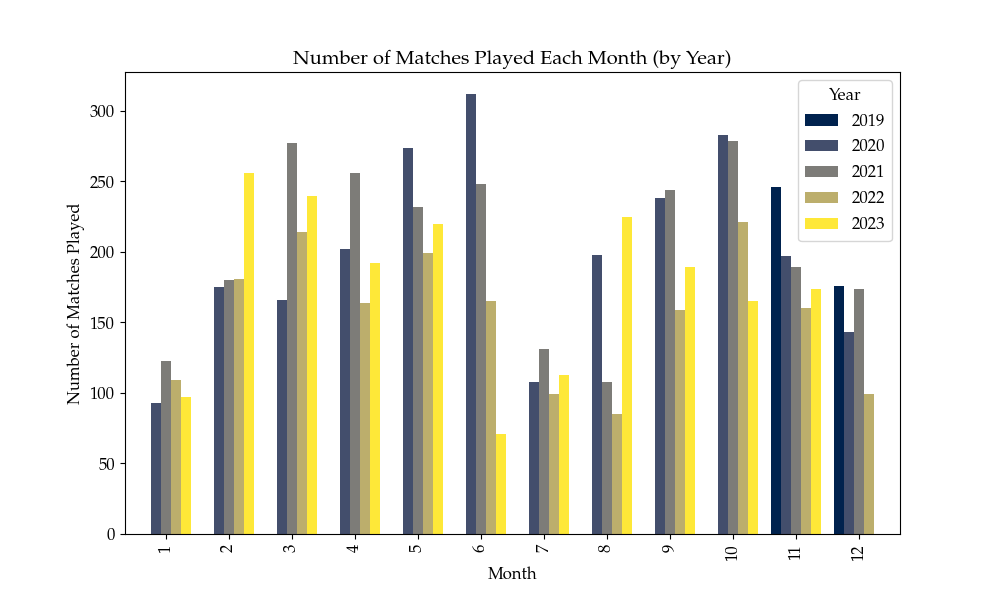
\includegraphics[width=1.3\textwidth]{Figures/matches-per-month-total.png}}
%	\caption{Distribution of matches player per month}
%	\label{fig:matches_per_month}
%\end{figure}
%
%\subsection{Game changes}
%
%Instead of releasing CS2 as a stand-alone title, Valve updated CS:GO on Steam, renaming it to CS2 and changing the game files. This meant that all players, both casual and professional, were forced to make the move to the new game on its release date of 27 September 2023. The first match of CS2 by a Top-50 team was played on 04 October 2023, and the last professional match of CS:GO ever played happened just a few days later on 10 October 2023.
%
%From a data analysis perspective, the biggest change between the titles was the introduction of MR12 (maximum rounds per half: 12). In CS:GO, maps were played in a best-of-30 (MR15) round format, however Valve decided to shorten games. This means that matches are shorter and each round contributes a greater share towards the win condition; only 13 round wins are required to win a map instead of the 16 in CS:GO. Overtime remained unchanged in best-of-6 format.



\subsection{Descriptive statistics}

The dataset is well-balanced, with 51.91\% of the match records having a class label of 1, and 48.09\% having a class label of 0. In other words, team 1 won 51.91\% of the matches and team 2 won 48.09\%. 

Plotting the distribution of different features for either target class is a useful way to visualize the extent to which features correlate with the target class. From Figure \ref{fig:win_prob_class_dist}, it is clear that TrueSkill makes more confident predictions than the Elo rating system, as the inter-quartile range is greater for both classes. The Elo rating system rates the majority of matches as being relatively even. The HLTV ranking difference refers to the value of team 2's rank less team 1's rank (a positive value indicates that team 1 had a higher rank than team 2). All three features exhibit larger median values for the winning class ($y=1$).

In each boxplot, values that are located 1.5 times the inter-quartile range below the first quartile and above the third quartile are considered outliers, and appear on the plot as hollow points.

\begin{figure}[h]
	\centering
	\begin{adjustbox}{center}
			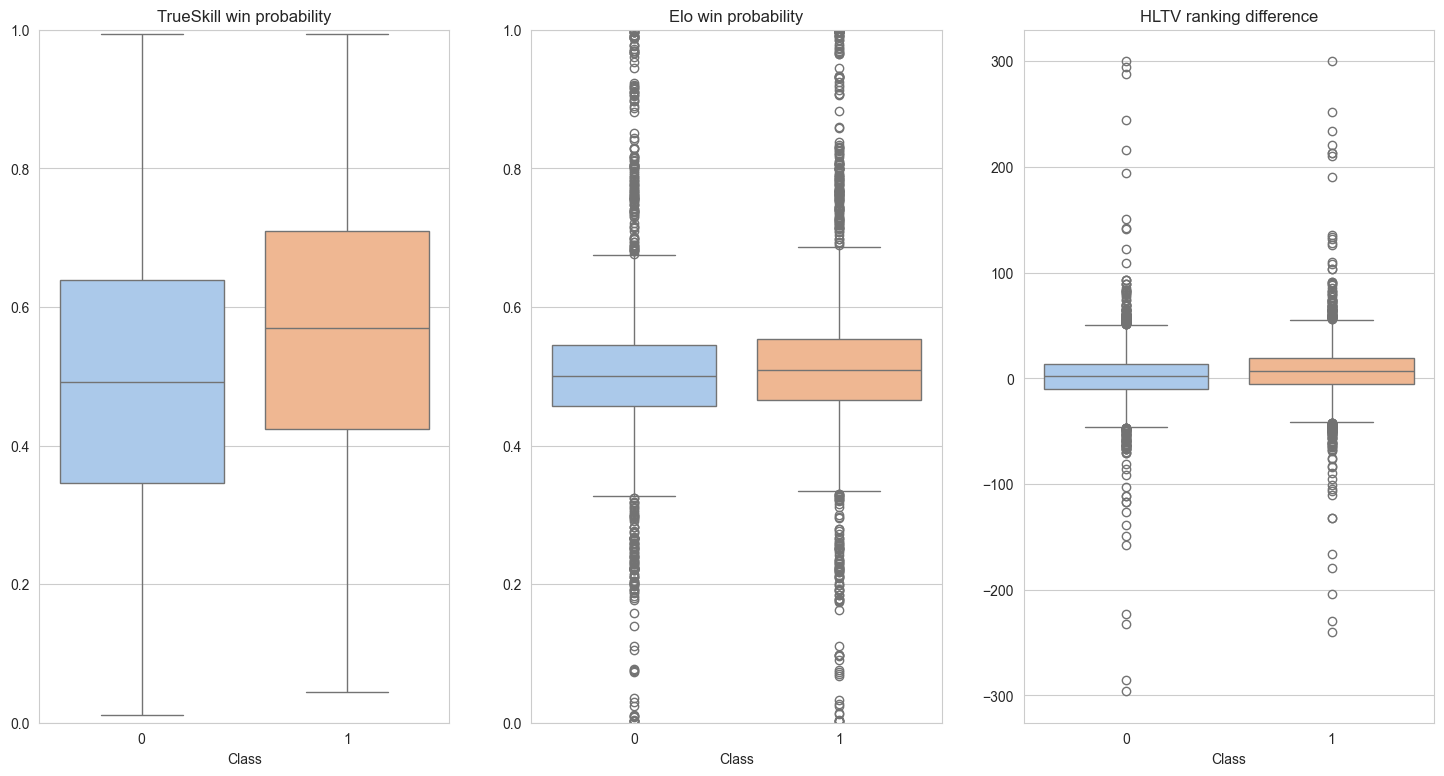
\includegraphics[width=1.2\textwidth]{Figures/class-box-new-1.png}
	\end{adjustbox}
	\caption{Boxplot of 'TrueSkill win probability', 'ELO win probability', and 'HLTV ranking difference' for either class}
	\label{fig:win_prob_class_dist}
\end{figure}

A similar trend is observed in Figure \ref{fig:win_rate_class_dist}, which plots the distribution of various win rates. The winning team generally had a higher overall win-rate for prior matches. The number of maps where a team had a higher win-rate can range from -7 to 7 (as there are seven maps in the competitive map pool). The median value was 1 indicating that the winning team usually had at least one more map with a higher win-rate than their opponent. The head-to-head historical map win-rate feature is also interesting, as there is a higher disparity between the classes. The conclusion that can be drawn here is that if team $x$ beat team $y$ more often than not in the past, they will likely continue to beat them in future. The IQR was, however, quite broad. Furthermore, for over 60\% of the matches, both teams had not played each other in the last 3 months.

\begin{figure}[h]
	\centering
	\begin{adjustbox}{center}
		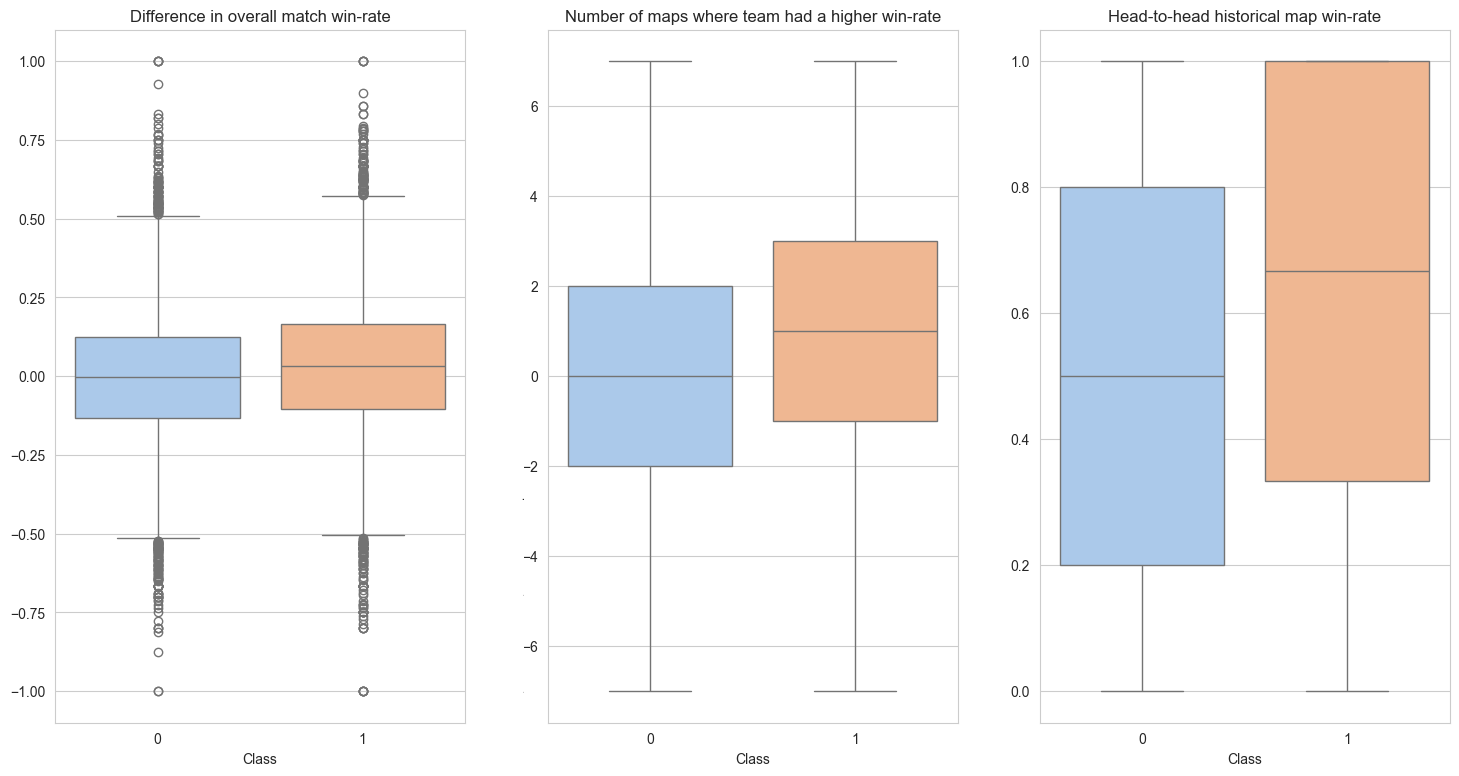
\includegraphics[width=1.2\textwidth]{Figures/class-box-new-2.png}
	\end{adjustbox}
	\caption{Boxplot of 'difference in match win-rate', 'maps with a higher win-rate', and 'head-to-head historical map win-rate' for either class}
	\label{fig:win_rate_class_dist}
\end{figure}

The most popular format in the dataset is BO3, with \matchesBoThree{} matches played (78.5\%). There were a further \matchesBoOne{} BO1s and \matchesBoFive{} BO5s played. The remaining 47 matches were played in BO2 maps, a format used briefly for lower-level league matches in 2019 and never again since. 

\matchesLAN{} (19.7\%) of the matches were played in a LAN environment, with the other \matchesOnline{} (80.3\%) being played online. 

Shortly after its release in September 2023, the professional scene transitioned to CS2. This meant that only \matchesCSTwo{} matches in the database were played in the new game, with the vast majority (\matchesCSGO{}) played in CS:GO. As the dataset grows in future, the proportion will shift in favour of CS2 matches. Nevertheless, the core game has remained unchanged, and the same analysis is applicable for both iterations of Counter-Strike.

\newpage

\subsection{Feature correlation}

It is useful to plot a correlation matrix to understand the relationships between pairs of variables. It can also help to identify multicollinearity, where independent variables are highly correlated. Highly correlated features essentially provide redundant information to a model, and can result in unstable and unreliable coefficient estimates. Dimensionality reduction techniques, such as principal component analysis, can be implemented to mitigate multicollinearity, however with the trade-off that new uncorrelated variables, called principal components, are less interpretable.

The correlation matrix for thirty of the features is plotted in Figure \ref{fig:corr}. It is immediately observable that none of the features correlate strongly with the target class \textit{win}. This is evident by the top row consisting of just pale colours. 

\begin{figure}[h]
	\centering
	\begin{adjustbox}{center} % Center the table
		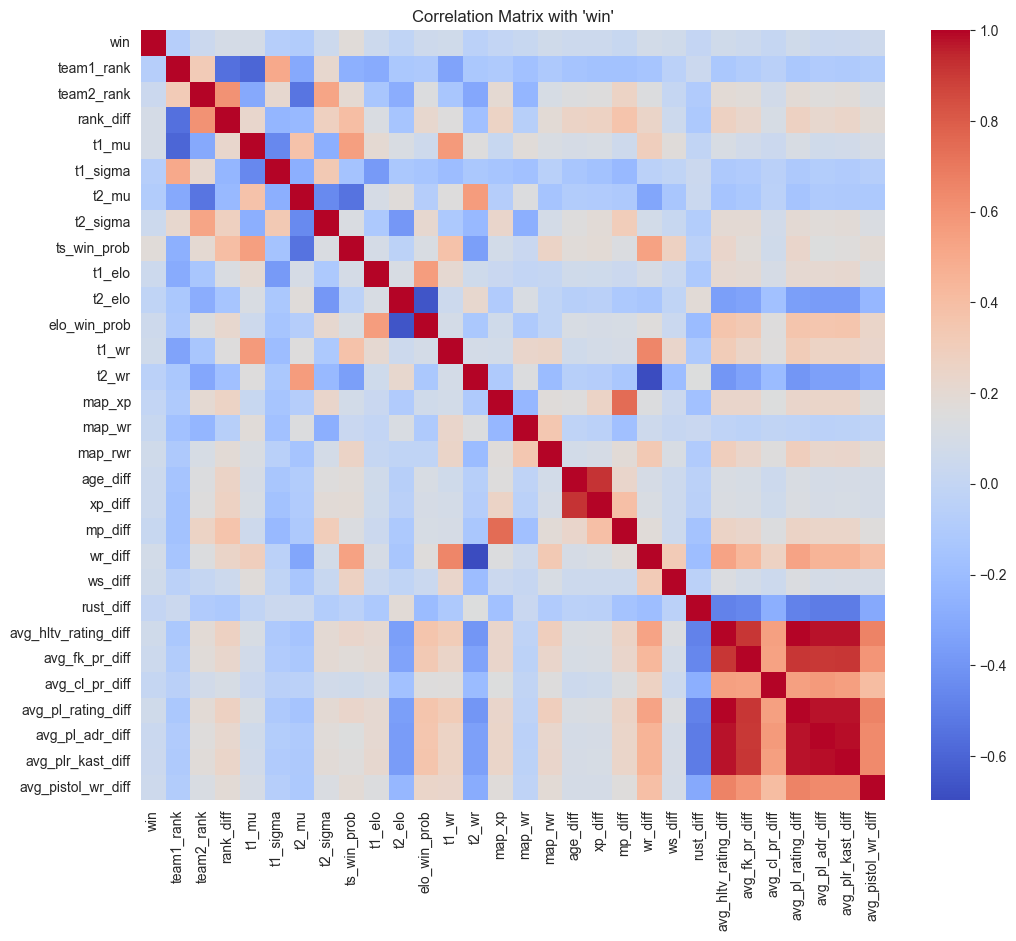
\includegraphics[width=1.3\textwidth]{Figures/corr-plot.png}
	\end{adjustbox}
	\caption{Feature correlation matrix heat-map}
	\label{fig:corr}
\end{figure}

\clearpage

A negative correlation between `team1\_rank' and 't1\_mu' exists, as well as for 'team2\_rank' and 't2\_mu'. This is a good indication that the TrueSkill system was implemented correctly. The best teams are ranked ascending from 1st, 2nd, 3rd - it is logical for teams with a low rank value to have a higher TrueSkill average ($\mu$). The TrueSkill averages correlate with their respective match win-rates.

Lineup age (measured in days) and experience (measured in number of matches together) also exhibit an unsurprising correlation. 

The red cluster in the bottom-right indicates a strong correlation between the  performance features. This is not too surprising because generally, having a high ADR or KAST will lead to a higher player rating, and having higher player ratings leads to a higher team rating. Furthermore, the more 'clutches' and 'first kills' obtained per round, the higher your team's overall performance will be.

% The number of maps and matches played each month and year
% distribution of match format (best of 1/2/3/5)
% distribution of maps played (mirage/inferno/etc)
% number of matches played by rank
% distribution of scores (13-0, 13-1, 13-2, 13-3, etc)
% score distribution and subsequent probability of winning (1-0, 2-0, 2-1, 3-1, 3-2, 4-0, 4-1, 4-2, 4-3, etc.)
% number of events, online/LAN, prizepools
% 1st pistol round win and map win (split by T/CT)
% 2nd pistol round win given each permutation of first half-score (split by T/CT)
% After winning opponent’s map pick, probability of winning series
% After winning your map pick, probability of winning series
% Matches won with rank differential

\subsection{Baseline model predictors}

\label{feature-selection}

It is useful to evaluate the performance of more basic models, with only 1 or 2 features, to form a baseline benchmark with which comparisons can be made. This will help to understand if the use of machine learning techniques offers a real benefit over a simpler analysis. To facilitate this, the most important features were identified via a feature selection process.

\textit{Feature selection} refers to the selection of the most relevant features from a dataset. It is used to reduce over-fitting and simplify models. Features can be selected either based on a statistical measure (a filter method), or by evaluating the performance of models using different subsets of features (a wrapper method).

A filter method was implemented using the \texttt{\textbf{f\_classif}} function from scikit-learn's \texttt{\textbf{feature\_selection}} class. By computing the ANOVA F-value, or \textit{F-statistic}, between each feature and the target class, each feature can be ranked and compared. The ANOVA F-value refers to the ratio of variance between the classes and the variance within the classes for each feature, thereby determining how well each feature can discriminate between each class, $y=0$ or $y=1$. If a feature has a higher ANOVA F-value, it has a stronger relationship with the target class and is potentially more useful for classification.

Other methods for feature selection were considered, such as \texttt{\textbf{SelectFdr}} which accounts for the family-wise error rate. However given the exploratory data analysis context, the filter method was deemed sufficient, and the best $k$ features or top $n^{th}$ percentile were identified using the \texttt{\textbf{SelectKBest}} function. The information presented in Figure \ref{fig:f-stat} was obtained by setting $k = 15$. 
\clearpage

\begin{figure}[h]
	\centering
	\begin{adjustbox}{center} % Center the table
		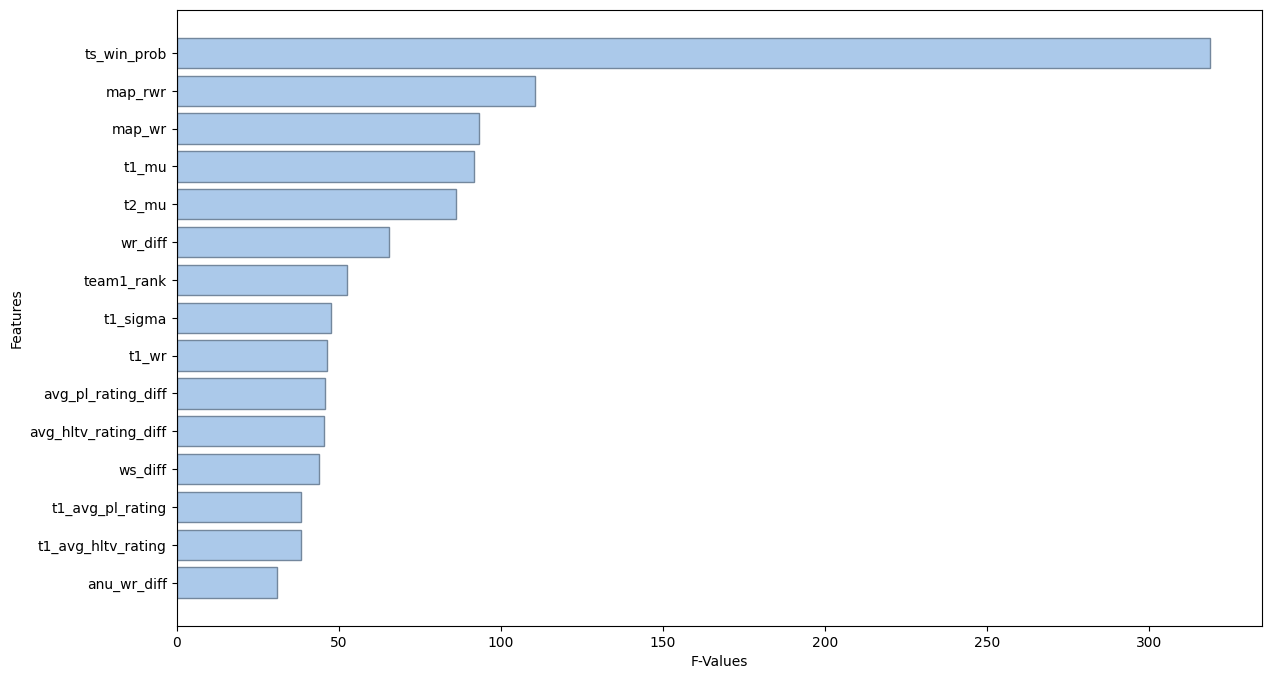
\includegraphics[width=1.3\textwidth]{Figures/f-statistik.png}
	\end{adjustbox}
	\caption{Barplot of best features by F-value}
	\label{fig:f-stat}
\end{figure}

The TrueSkill features appear to be the best predictors of the match outcome, with the win probability and mean $\mu$ values for either team exhibiting the highest scores. The map win-rate differential, round win-rate differential, and HLTV world ranking all follow, but with a large drop-off in score.

From these insights, we can establish three baseline models:

\begin{enumerate}
	\item the TrueSkill win probability model
	\item the HLTV world ranking model, where the team with the higher rank is always predicted to win
	\item the map win-rate model, where the team with the higher win-rate on more maps is always predicted to win. If both teams are equal, then the team with the higher overall round win-rate on more maps is predicted to win.
\end{enumerate}

\textbf{TrueSkill} achieved a classification accuracy of 57.00\% on the full dataset of \matchesTotal{} matches. The confusion matrix is shown in Table \ref{tab:ts-conf}. 

From the matrix, a number of useful statistics can be computed. The true positive rate (TPR, also known as sensitivity or recall) is the proportion of actual positives correctly identified by the model. The true negative rate (TNR, also known as specificity) is the proportion of actual negatives correctly identified by the model. Precision refers to the proportion of positive classifications that were correct. The F1-score is a balanced measure of precision and recall. These metrics will be discussed in more depth later. The TrueSkill model achieved a true positive rate of 0.62, a true negative rate of 0.516, a precision of 0.58, and a F1-score of 0.60.

\begin{table}[h]
	\centering
	\begin{tabular}{c|c|c|}
		\cline{2-3}
		& \textbf{Predicted: No} & \textbf{Predicted: Yes} \\ \hline
		\multicolumn{1}{|c|}{\textbf{Actual: No}} & 2516 & 2363 \\ \hline
		\multicolumn{1}{|c|}{\textbf{Actual: Yes}} & 1999 & 3267 \\ \hline
	\end{tabular}
	\caption{Confusion matrix for the TrueSkill model}
	\label{tab:ts-conf}
\end{table}

TrueSkill can evaluate the probability of a team winning, which means a receiver operating characteristic curve can be constructed by varying the threshold at which this probability is enough to make a positive classification. The area under the receiver operating characteristic curve (AUC ROC) is a measure of classifier's ability to distinguish between the two classes. As shown in Figure \ref{fig:ts-roc}, the TrueSkill model is indeed a better predictor than random chance, with the area under the curve, $AUC = 0.5997$. The probabilities generated by TrueSkill may also be converted into betting odds. This aspect will be discussed later.
 
\begin{figure}[h]
	\centering
	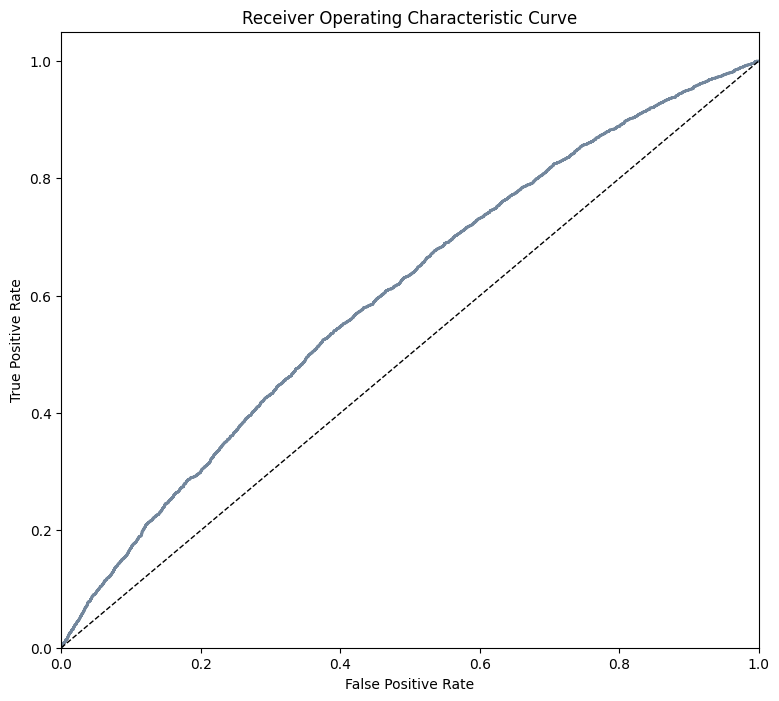
\includegraphics[width=\textwidth]{Figures/ts-auc.png}
	\caption{ROC curve for the TrueSkill model}
	\label{fig:ts-roc}
\end{figure}

The \textbf{HLTV world ranking model}, which assumes the higher-ranked team will always win the match, correctly classified the winner for 56.28\% of the matches, achieving a slightly higher F1-score than TrueSkill of 0.61. The final baseline model, the \textbf{map win-rate model}, achieved only 54.95\% classification accuracy and a lower F1-score of 0.579. As neither of these last two models produce classification probabilities, no receiver operating characteristic curve can be constructed.

\section{Modelling}

After considering the methods used in the literature, the following supervised learning models were selected and trained to predict the match winner:

\begin{itemize}
	\item Logistic regression
	\item Random forests
	\item Support vector machine
	\item $k$-nearest neighbours
	\item Gaussian Naive Bayes
	\item Multilayer perceptron
	\item XGBoost
\end{itemize}

\subsection{Data segmentation}

To accurately assess the performance of any ML model, it must be tested on data which has not been used during training. The data should therefore be split into a training set and a testing set. Because the match data is chronological time-series data, it would not be appropriate to randomise the data prior to splitting, which is a common practice. It is more appropriate to segment the data chronologically.

A portion of the earliest match data was excluded from both training and testing. These matches were used to generate features for the later matches. This served two main purposes: the initialisation of Elo and TrueSkill ratings, and for providing historical data for most of the match- and performance-history features. This initialisation set amounted to the first 10\% of the dataset, which was 1127 matches spanning a period of five months. This ensured that the features generated for the first match in the training set could draw upon accurate player ratings and sufficient match history for each team.

The remaining 90\% of the data shall henceforth be referred to as the \textit{full dataset}. It was split with a ratio of 80:20 for the training and testing sets. The test set consisted of every match played in 2023. This amounted to 8116 match records for training and 2029 for testing.

Filters were later applied to the full dataset in order to identify if certain types of matches were easier to predict than others. The different scenarios tested were:
\begin{enumerate}
	\item the full dataset,
	\item a dataset which excluded all Best-of-1 (single map) matches,
	\item a dataset which excluded matches without a team ranked in the Top-30,
	\item a dataset which excluded matches without a team ranked in the Top-15, and
	\item a dataset which excluded all matches which were played online (i.e. LAN matches only)
\end{enumerate}

The same process was performed for each dataset: data segmentation, feature scaling, feature selection, hyperparameter tuning, and performance evaluation.

\subsection{Feature scaling}

Some models, such as those which use gradient descent for optimisation, are sensitive to the magnitude of features. This means that each numeric feature should be \textit{scaled} prior to training. There are two methods of scaling features, namely \textit{normalisation} and \textit{standardisation}. In normalisation, each feature is scaled to fit into the range $[0, 1]$ by subtracting the minimum value and dividing by the range, ($max-min$). Although normalised data preserves the distribution of the original data, it is more sensitive to outliers. 

In standardisation, the data is transformed to have a zero mean and unit variance using the familiar equation:

\[ z_i = \frac{x_i-\mu}{\sigma} \]

Where $z_i$ is the new value, $x_i$ is the original value, $\mu$ and $\sigma$ are the mean and standard deviation of $x$.

Both techniques were implemented using the \texttt{\textbf{MinMaxScaler}} and \texttt{\textbf{StandardScaler}} classes from scikit-learn. During testing, it was found that normalisation degraded model performance significantly when compared to both the unscaled and standardised data. This is because normalisation is sensitive to outliers, which were present in many of the features. It was therefore decided to scale the features using standardisation. 

\subsection{Hyperparameter tuning}

Each ML model has configuration settings which dictate the structure and computational performance of the model. These settings are known as \textit{hyperparameters}. An example of a hyperparameter is the maximum depth of the decision trees used in random forests, or the choice of kernel used in a SVM.

When tuning these parameters to find the optimal configuration, it is a good practice to partition a portion of the training set into a validation set. The performance of models with different configurations can be compared by testing them on the validation set.

A technique known as $k$-fold cross-validation splits the training data into $k$ folds (partitions). The training is then performed repeatedly with a different fold used as the validation set for each iteration. This approach provides a proxy for estimating the out-of-sample performance, ensuring that a balanced measure of performance is attained for each configuration of hyperparameters.

The \texttt{\textbf{GridSearchCV}} class from scikit-learn was utilized to test several different hyperparameters grids (configurations) using $k$-fold cross-validation. For many of the hyperparameters, a broad initial range of values was used. This range was progressively narrowed down in an iterative process until the configuration yielding the greatest average classification accuracy on the validation set was found.

The hyperparameters for each method and the range of values considered are explained in the following subsections.

\subsubsection{Logistic regression}

Table \ref{tab:lr_params} presents the hyperparameters of the logistic regression model and the respective ranges of values explored during the tuning process.

\begin{table}[h]
	\centering
	\begin{tabular}{ll}
		\toprule
		\multicolumn{1}{c}{\textbf{Hyperparameter}} & \multicolumn{1}{c}{\textbf{Values Tested}} \\
		\midrule
		1/Regularisation strength (C)              & $10^{-5}$ - $10^{2}$ \\
		Regularisation type                       & None, L1 (Lasso), L2 (Ridge) \\
		Solver                                    & liblinear, lbfgs, saga \\
		\bottomrule
	\end{tabular}
	\caption{Logistic regression hyperparameters and the range of values tested}
	\label{tab:lr_params}
\end{table}

Regularisation introduces a penalty term to the loss function which helps control the size of the coefficients. This can mitigate the risk of overfitting by preventing the model from relying too heavily on any single predictor variable. There are two \textit{types} of regularisation, Lasso and Ridge.

$C$ is the inverse of the \textit{regularisation strength} parameter $\lambda$. Higher values of $C$ therefore correspond to less regularisation, while lower values enforce stronger regularisation.

The \textit{solver} is the algorithm used to minimise the loss function. 

\subsubsection{Random forests}

Table \ref{tab:rf_params} presents the hyperparameters of the random forests model and the respective ranges of values used in the tuning process.

\begin{table}[h]
	\centering
	\begin{tabular}{ll}
		\toprule
		\multicolumn{1}{c}{\textbf{Hyperparameter}} & \multicolumn{1}{c}{\textbf{Values Tested}} \\
		\midrule
		Number of estimators       & 20 - 500 \\
		Maximum depth              & 2 - None \\
		Minimum samples for split  & 2 - 10 \\
		Minimum samples per leaf   & 1 - 10 \\
		Maximum features           & 1 - None \\
		\bottomrule
	\end{tabular}
	\caption{Random forests hyperparameters and the range of values tested}
	\label{tab:rf_params}
\end{table}

The \textit{number of estimators} is the number of decision trees to include in the ensemble. Increasing this value can improve performance but also increases computational cost.

The \textit{maximum depth} limits the maximum depth of each decision tree. Deeper trees can capture more complex relationships but may overfit the data. 

The \textit{minimum samples for split} are the amount of samples needed at a node in order to split it further. The \textit{minimum samples per leaf} are the lowest amount of samples that can exist at a leaf node. The greater these values, the simpler the trees become.

The \textit{maximum features} refers to the maximum amount of features considered when looking for the best split. Limiting the number of features reduces the risk of overfitting.

\subsubsection{Support vector machine}

Table \ref{tab:svc_params} presents the hyperparameters of the support vector machine and the respective ranges of values explored during the tuning process.

\begin{table}[h]
	\centering
	\begin{tabular}{ll}
		\toprule
		\multicolumn{1}{c}{\textbf{Hyperparameter}} & \multicolumn{1}{c}{\textbf{Values Tested}} \\
		\midrule
		Kernel                     & 'linear', 'poly', 'rbf', 'sigmoid' \\
		Regularisation (C)         & $10^{-3}$ - $10^{3}$ \\
		Degree (for 'poly' kernel) & 2 - 5 \\
		Gamma (for 'rbf' kernel)   & $10^{-5}$ - $10^{0}$ \\
		\bottomrule
	\end{tabular}
	\caption{Support Vector Classifier hyperparameters and the range of values tested}
	\label{tab:svc_params}
\end{table}

The \textit{kernel} function defines the shape of the decision boundary.

For a support vector classifier, Ridge regularisation is implemented by means of a penalty term for the complexity of the decision boundary. The \textit{regularisation} parameter C is the inverse of the strength of regularisation, where lower values of C correspond to stronger regularisation, while higher values correspond to weaker regularisation

For the polynomial kernel, the \textit{degree} specifies the polynomial order, and for the RBF kernel, the \textit{gamma} parameter defines the kernel width.

\subsubsection{\textit{k}-nearest neighbours}
Table \ref{tab:knn_params} presents the hyperparameters of the $k$-nearest neighbours classifier and the respective ranges of values explored during the tuning process.

\begin{table}[h]
	\centering
	\begin{tabular}{ll}
		\toprule
		\multicolumn{1}{c}{\textbf{Hyperparameter}} & \multicolumn{1}{c}{\textbf{Values Tested}} \\
		\midrule
		Number of neighbours			   & 1 - 30 \\
		Weight function			           & 'uniform', 'distance' \\
		Algorithm                          & 'auto' \\
		Power parameter (p)                & 1 - 2 \\
		\bottomrule
	\end{tabular}
	\caption{$k$-nearest neighbours hyperparameters and the range of values tested}
	\label{tab:knn_params}
\end{table}

The \textit{number of neighbours} are the number of neighbouring data points which are considered for classification. A higher value can reduce noise but may also smooth out decision boundaries.

The \textit{weight function} assigns a weight to each neighbour based on its distance from the query point. 'uniform' gives equal weight to all neighbours, while 'distance' weights closer neighbours more heavily.

The \textit{algorithm} parameter specifies the algorithm used for computing nearest neighbors. 'auto' selects the best approach based on the dataset.

The \textit{power} parameter (p) is used for the Minkowski metric, which calculates the distance between data points. The Manhattan distance is used when $p=1$, and the Euclidean distance is used when $p=2$.

\subsubsection{Gaussian Naive Bayes}

The Gaussian Naive Bayes classifier is a relatively simple model and has only a single hyperparameter, \textit{var\_smoothing}, which is a small positive value added to the variance of each Gaussian used in the model. Adding this smoothing value can prevent numerical instabilities if the variance of a feature approaches 0. The range of values tested was $10^{-10}$ - $10^{-5}$.

\subsubsection{Multilayer perceptron}

Table \ref{tab:mlp_params} presents the hyperparameters of the MLP classifier and the respective ranges of values explored during the tuning process.

\begin{table}[h]
	\centering
	\begin{tabular}{ll}
		\toprule
		\multicolumn{1}{c}{\textbf{Hyperparameter}} & \multicolumn{1}{c}{\textbf{Values Tested}} \\
		\midrule
		Hidden layer sizes  				& \textit{see below} \\
		Activation function 				& 'identity', 'logistic', 'tanh', 'relu' \\
		Solver 								& 'lbfgs', 'sgd', 'adam' \\
		Learning rate 						& 'constant', 'invscaling', 'adaptive' \\
		Alpha 								& 0.0001, 0.001, 0.01, 0.1 \\
		Batch size 							& 'auto', 20 - 400 \\
		Max iterations					    & 200 - 10000 \\
		\bottomrule
	\end{tabular}
	\caption{Multilayer perceptron hyperparameters and the range of values tested}
	\label{tab:mlp_params}
\end{table}

The \textit{hidden layer sizes} are the number of neurons in each hidden layer. Different configurations of hidden layers can affect the model's ability to capture complex patterns. The hidden-layer topologies tested include wide (200,200), narrow (20,20), bottleneck (200, 50, 200), and hierarchical (200, 100, 50). The amount of neurons in each hidden layer in each topology was varied from 1 to 400. The maximum number of hidden layers tested was five.

The \textit{activation function} defines the function used for activating neurons in the hidden layers, where 'identity' is a linear activation, 'logistic' is the sigmoid function, 'tanh' is the hyperbolic tangent, and 'relu' is the rectified linear unit.

The \textit{solver} is the optimization algorithm used to update the weights. 'lbfgs' is an quasi-Newton method, 'sgd' is stochastic gradient descent, and 'adam' is a stochastic gradient-based optimizer.

The \textit{learning rate} controls the step size used when updating the weights. 'constant' uses a fixed learning rate (0.001), 'invscaling' gradually decreases the learning rate, and 'adaptive' maintains the learning rate unless the training loss ceases to improve.

The \textit{alpha} parameter is the regularisation term, similar to $\lambda$ in logistic regression and SVMs.

The \textit{batch size} is the number of samples processed before the model is updated. Smaller batch sizes allow the model to learn faster but can be more unstable, while larger batch sizes provide more stable updates but may take longer to converge.

The \textit{max iterations} parameter is the maximum number of iterations the solver will run for. This allows "early stopping" if convergence is not reached after max\_iter. For stochastic solvers (‘sgd’, ‘adam’), this is the number of times each data point is used (epochs).

\subsubsection{XGBoost}
Table \ref{tab:xgb_params} presents the hyperparameters of the XGBoost classifier and the respective ranges of values explored during the tuning process.

\begin{table}[h]
	\centering
	\begin{tabular}{ll}
		\toprule
		\multicolumn{1}{c}{\textbf{Hyperparameter}} & \multicolumn{1}{c}{\textbf{Values Tested}} \\
		\midrule
		Number of estimators	  				  & 50 - 10000 \\
		Learning rate        					  & 0.001, 0.01, 0.1, 0.2, 0.3 \\
		Max depth            					  & 2 - 10 \\
		Subsample 								  & 0.5 - 1.0 \\
		Colsample by tree 					 	  & 0.5 - 1.0 \\
		Gamma 									  & 0, 0.1, 0.2, 0.3 \\
		\bottomrule
	\end{tabular}
	\caption{XGBoost hyperparameters and the range of values tested}
	\label{tab:xgb_params}
\end{table}

The \textit{number of estimators} is the number of trees in the model. More trees can increase the model's performance but also the risk of overfitting.

The \textit{learning rate} (eta) controls the step size at each iteration while minimising the loss function. Lower learning rates make the model more robust to overfitting by shrinking the feature weights.

The \textit{max depth} parameter defines the maximum depth of a tree. Deeper trees can model more complex relationships but are more prone to overfitting.

The \textit{subsample} parameter is the fraction of samples to be used for fitting each tree, while \textit{colsample by tree} is the fraction of features to be used for each tree. These parameters prevent overfitting by adding randomness.

The \textit{gamma} parameter specifies the minimum reduction in loss needed to split a node, thereby controlling the complexity of the trees.
 
\subsection{Performance evaluation}

Once each model has been trained, each match in the test set is classified into either class, $y=1$ (team 1 wins), or $y=0$ (team 1 loses, i.e. team 2 wins). 

The classification accuracy refers to the percentage of matches that was correctly classified by each model. It is reported as \textbf{Test ACC} in the results tables in the following chapter. 

\textbf{Precision} is a measure of the accuracy of positive predictions. It is the percentage of matches that were actually won out of the set of positive predictions. \textbf{Recall}, also known as sensitivity, measures the proportion of true positives that are correctly classified by the model.

\[ \text{Precision} = \frac{\text{True Positives}}{\text{True Positives} + \text{False Positives}} \]
\[ \text{Recall} = \frac{\text{True Positives}}{\text{True Positives} + \text{False Negatives}} \]

\textbf{F1-score} is another measure of predictive performance which balances both precision and recall. 

\[ F_1 = \frac{2 \times precision \times recall}{precision + recall} \]

Finally, the \textbf{area under receiver operating characteristic curve} (AUC ROC) is a measurement of the classification performance of a model at different threshold settings. The ROC curve plots the True Positive Rate (recall) against the False Positive Rate as the discrimination threshold is varied from 0 to 1. A random classifier will therefore, on average, have a straight line from (0,0) to (1,1) with a corresponding AUC ROC of 0.5. An AUC ROC of 1.0 indicates that the model can perfectly distinguish the positive and negative classes.

\subsection{Betting odds generation}

Each of the models generate the probability $p(y)$ of an observation belonging to each class. These probabilities are then used to generate the betting odds. Odds can be represented in a number of ways. For this research, all odds are denoted as decimal odds, which is a decimal number representing the payout per unit wagered. 

The decimal odds are the reciprocal of the probability of the event occurring as shown in the following equation:

\[ \left( O_A, O_B \right)  = \left( \frac{1}{p(y=1)}, \frac{1}{p(y=0)} \right) \]

Where $O_A$ and $O_B$ are the decimal odds for team A and B to win the match, and $p(y)$ is the probability of team A winning $(y=1)$ or team B winning $(y=0)$. In practice, these odds represent the \textit{fair} odds which exclude the effect of the bookmaker margin: a reduction in the decimal odds to increase bookmaker profitability.

\newcommand{\matchesBet}{347}
\newcommand{\tournamentsBet}{11}

\subsection{Betting odds evaluation}

In order to compare the generated betting odds with real betting odds provided by bookmakers, the average odds for \matchesBet{} matches across \tournamentsBet{} tournaments in the test set (2023) were downloaded from an online archive at \texttt{oddsportal.com}. To remove the bookmaker margin, the odds were then converted back into probabilities and normalized such that the sum of each pair of probabilities added up to 1.

The correlation, mean absolute error (MAE), and root mean square error (RMSE) between the generated odds and the bookmaker odds is reported for each model to quantify the discrepancy between the odds from the models and the bookmaker. These are formulated as follows:\label{bettingstats}

Given that the generated odds are $O_g$ and the bookmaker odds are $O_b$, with $n$ being the total number of odds comparisons, the \textbf{correlation} is defined as:

\[r = \frac{\sum_{i=1}^{n} (O_{g_i} - \bar{O_g})(O_{b_i} - \bar{O_b})}{\sqrt{\sum_{i=1}^{n} (O_{g_i} - \bar{O_g})^2 \sum_{i=1}^{n} (O_{b_i} - \bar{O_b})^2}}\]

where:
\begin{itemize}
	\item $O_{g_i}$ and $O_{b_i}$ are the i-th generated and bookmaker odds, respectively.
	\item $\bar{O_g}$ and $\bar{O_b}$ are the means of the generated and bookmaker odds.
\end{itemize}

The \textbf{mean absolute error} (MAE) is defined as:
\[\text{MAE} = \frac{1}{n} \sum_{i=1}^{n} |O_{g_i} - O_{b_i}|\]

And finally, the \textbf{root mean square error} (RMSE) is defined as
\[\text{RMSE} = \sqrt{\frac{1}{n} \sum_{i=1}^{n} (O_{g_i} - O_{b_i})^2}\]

\subsection{Betting simulation}

Finally, a betting simulation was performed to test each model's real-world performance using the following basic strategy: the bookmaker odds for each match was first converted into a probability. If the model generated a higher probability for either team to win than what was offered by the bookmaker, a one unit bet was placed on that team. 

For example, consider a scenario where the bookmaker odds for team A : team B is 1.28~:~3.36. These odds correspond to $p(y=1)=0.78$ and $p(y=0)=0.30$ (the sum is greater than 1 because of the bookmaker margin).

If the model then predicts that $p(y=1)=0.65$ and $p(y=0)=0.35$ for this match, it would place a one unit bet on team B, despite it having a lower probability of winning. 

On the other hand, if it had generated $p(y=1)=0.75$ and $p(y=0)=0.25$, it has determined that neither team is worth betting on.

The proportion of matches bet on, win-percentage, loss-percentage, and resulting profit or loss for each model is reported in the Results. 